{\section{Wnioski}}

Ćwiczenie polegało na wyznaczeniu przyspieszenia ziemskiego stosując zależności między przyspieszeniem,
a obiektami fizycznymi. Ćwiczenie zostało wykonane poprawnie.\\

Średnia wartość przyspieszenia jaka została zmierzona za pomocą wahadła matematycznego w budynku A-1 w sali 54 wyniosła $g = 9.91 \frac{m}{s^2}$.

\begin{figure}[h]
    \centering
    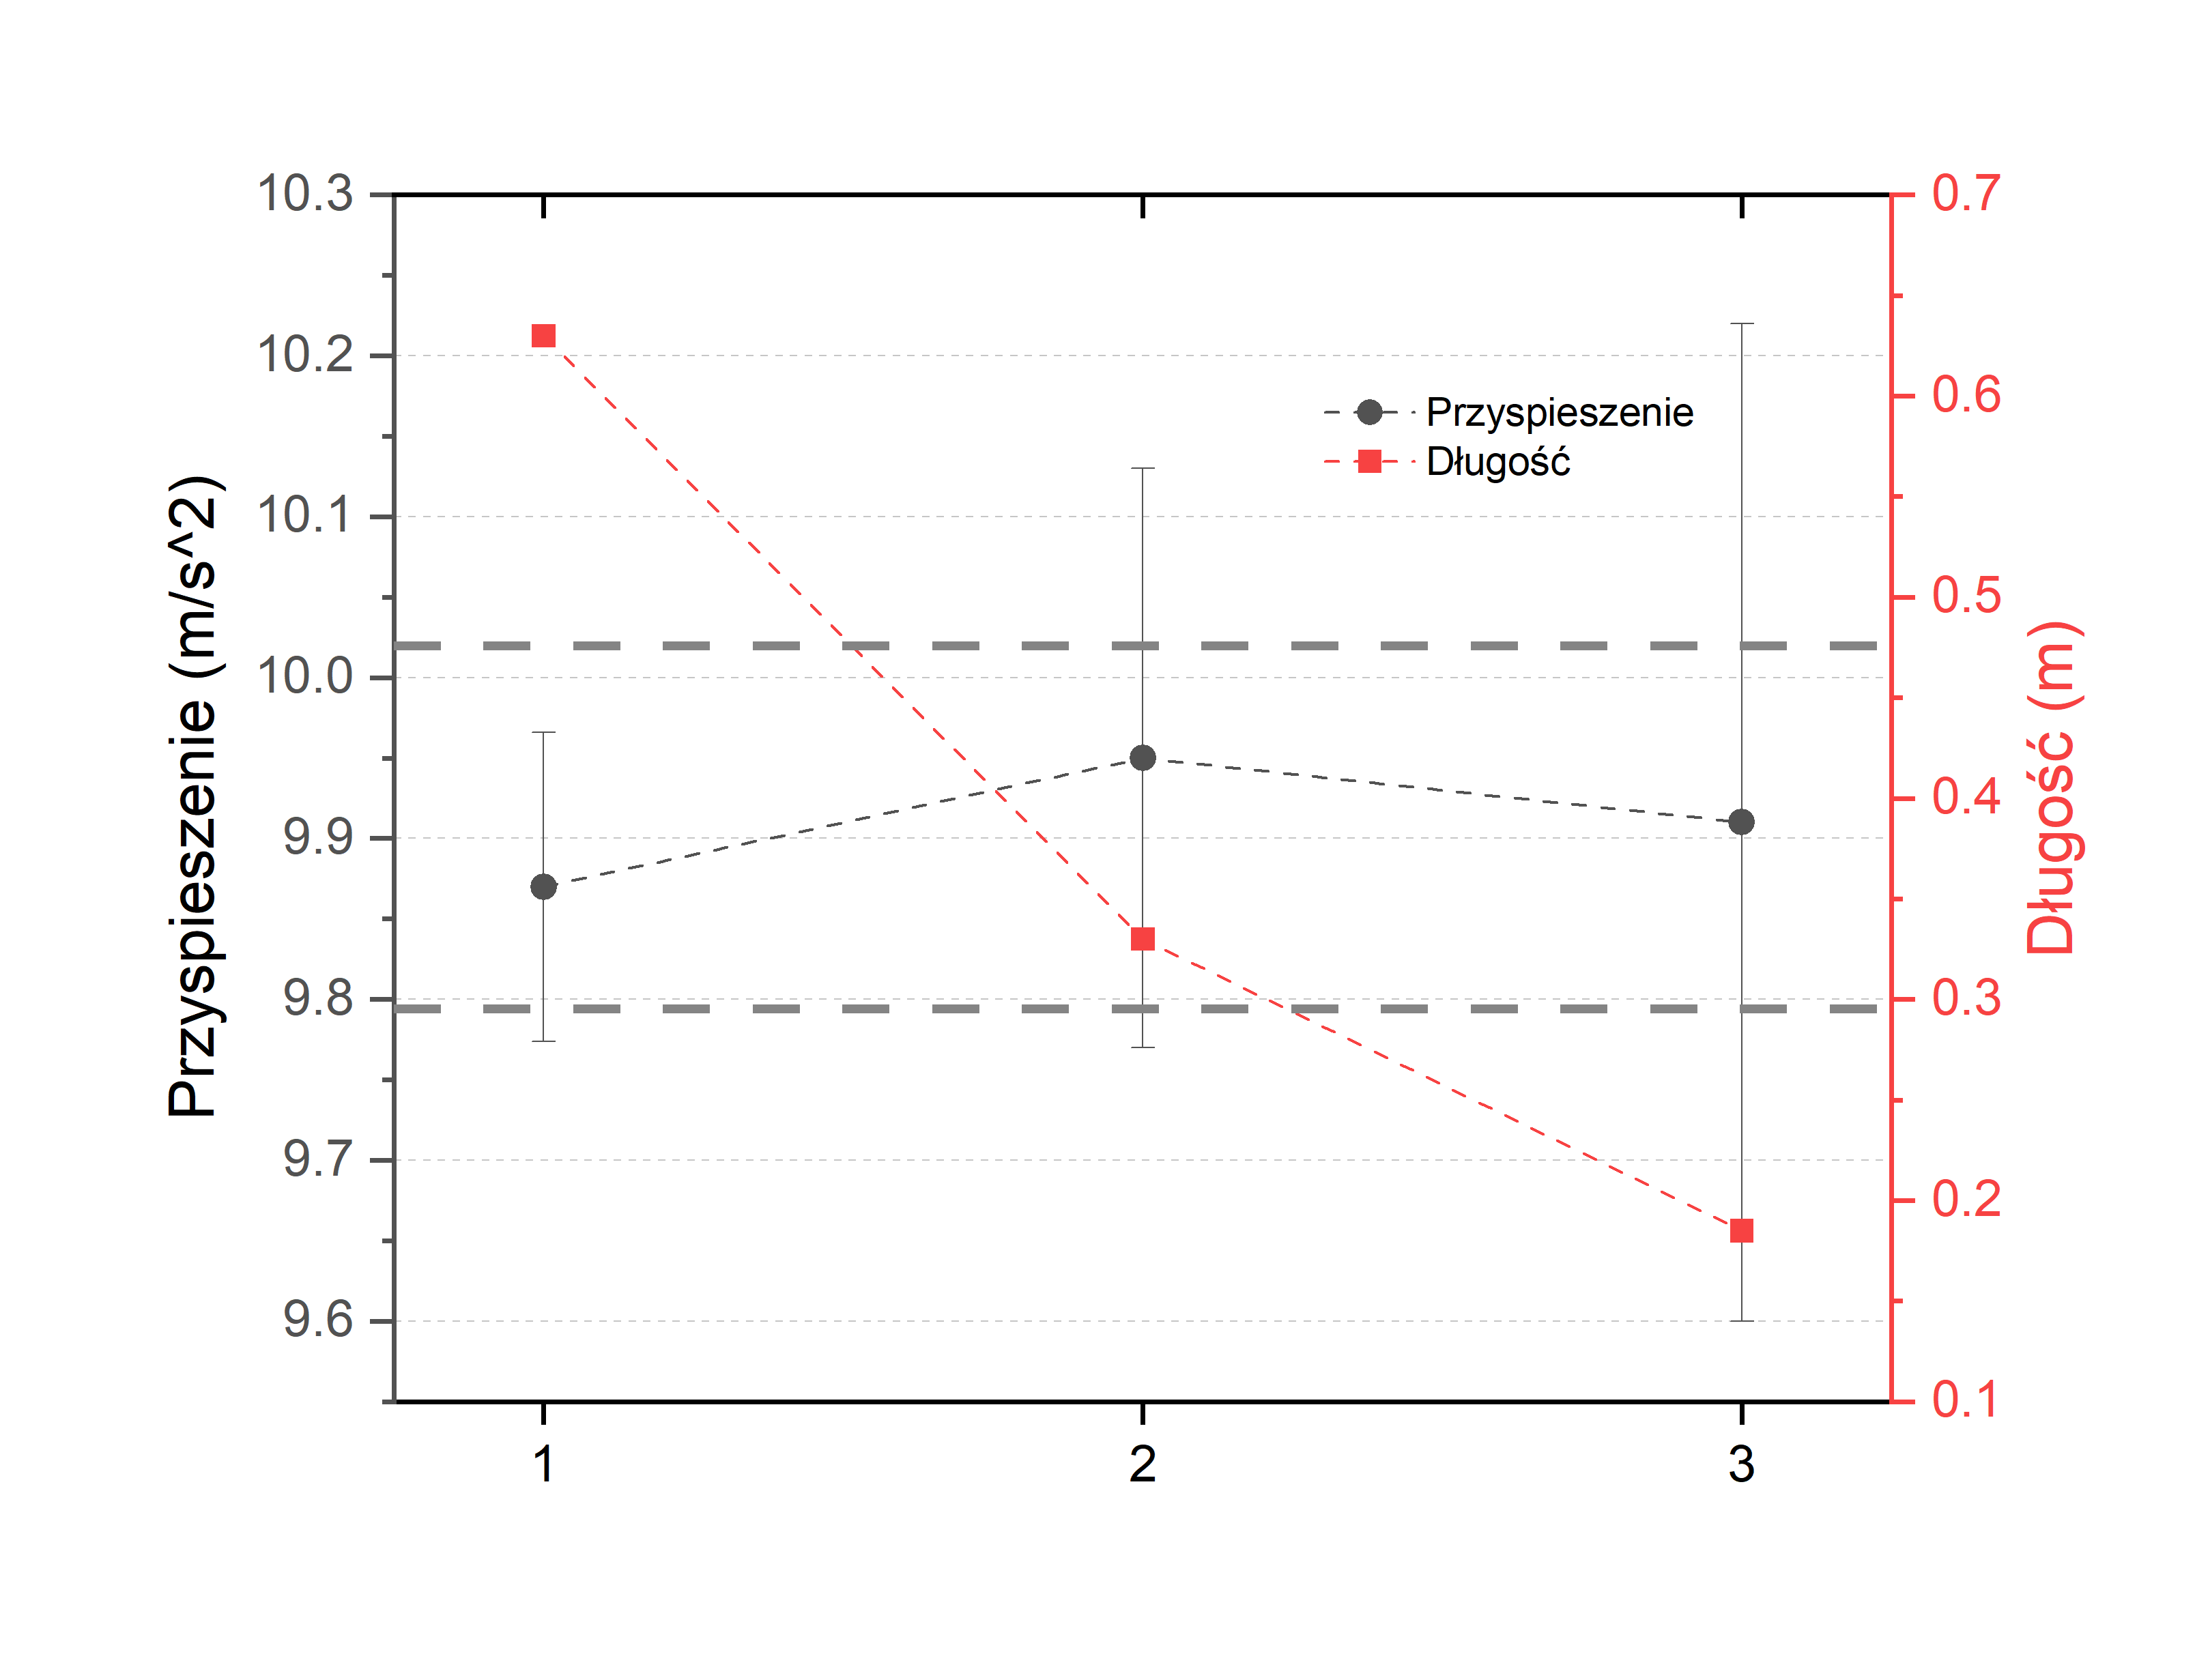
\includegraphics[width=100mm]{imgs/Graph1.png}
    \label{fig:wyniki_wm}
\end{figure}

Po zestawieniu obok siebie danych na wykresie można zauważyć pewną zależność między długością wahadła, a końcowym wynikiem ćwiczenia. Wszystkie 3 wyniki przyspieszenia ziemskiego dla poszczególnych długości wahadła mieszczą się w otoczeniu (niepewności) średniej ich wartości. Natomiast wraz ze skracaniem długości wahadła diametralnie wzrósła niepewność tego wyniku. Może to skutkować zbyt krótkim czasem oscylacji wahadła.

Wnioskujemy więc, że dla bardziej dokładnego wyniku przyspieszenia powinno się dokonywać doświadczenia stosując duże długości wahadła. Z zebranych danych wynika, że dla $l \leq 63cm$ otrzymamy dłuższe czasy oscylacji i większe uśrednienie okresu, co w efekcie końcowym da dokładniejszei wyniki przyspieszenia. \\

Średnia wartość przyspieszenia jaka została zmierzona za pomocą wahadła fizycznego w budynku A-1 w sali 54 wyniosła $g =10.26 \frac{m}{s^2}$.\\

Porównując te wyniki możemy wyciągnąć wniosek, że wahadło matematyczne  jest dokładniejszym narzędziem do wyznaczania wartości przyciągania grawitacyjnego.
